\chapter{Methods}
In this thesis, I analyze a dataset comprising the properties of a sample of galaxies from the Seventh Data Release (DR7) of the Sloan Digital Sky Survey. Covering 11,663 square degrees of imaging data, DR7 offers extensive five-band photometry for 357 million celestial objects \cite{2009ApJS..182..543A,mpa-sdss-dr7}. 

With completed spectroscopy over 9380 square degrees, including 1.6 million spectra of galaxies, quasars, and stars, the SDSS DR7 dataset serves as the primary catalog for this study.
 
Specifically i will focus on following physical properties : \textbf{Redshift} and \textbf{Integrated flux with their relative uncertainties} of the common optical lines (i.e. $H\alpha$, $H\beta$...).

In the context of SDSS DR7, the line-fitting process is divided into three main stages during an automated Gaussian fitting procedure applied to continuum subtracted data as follows :
\begin{enumerate}
\item The first stage involves fitting to only emission lines, referred to as "foundLines," and is performed during the determination of emission line redshifts.

\item The second stage, termed "measuredLines," represents the final fitting of all lines, including both emission and absorption lines. This stage occurs after the object has been classified, and the redshift has been determined.
\end{enumerate}
It is important to note that \textbf{each} line is \textbf{individually fitted as a single Gaussian} on the continuum-subtracted spectrum, with modalities shown in \cite{1994ApJ...422..158O}.

For the latter Radio identification i also use photometric informations, as later presented.
%FINO A QUI SOPRA SEMBRA OK 
 
%COMMENTI DI ANDREA
 \begin{comment}
 Specifically, I will focus on…. 


BREVEMENTE:
devi dire che utilizzi le seguenti proprietà: 
integrated flux and relative uncertainties of the common optical emission lines, i.e.,,,
(spiega come sono state derivate)
,redshifts (spiega con quale riga sono stati derivati)

Il redshift è lo shift verso il rosso dovuto perlopiù all’espansione dell’universo.
Si calcola solitamente avendo la lambda della riga osservata (lamb_obs), la lambda della riga osservata in laboratorio, quindi aspettata dalla teoria (lamb_exp) e si calcola come:

z = (lamb_obs/lamb_exp) -1

solitamente si usano righe come l’Hbeta o Halpha stretto. Ancora meglio righe molecolari. Vedi che hanno usato loro e dillo-.

Poi dì anche che sfrutterai informazioni fotometriche nel radio.

comunque andrai a parlarne dopo nel dettaglio 
\end{comment}
%VERSIONE INIZIALE CHE AVEVO MESSO IO
\begin{comment}
The study of cosmic objects, such as galaxies, relies on the analysis of the electromagnetic spectrum emanating from these distant sources. Within a spectrum, various pieces of information can be extracted, with the primary focus being on the intensity of light across a range of energies or frequencies. A crucial aspect of a spectrum involves determining the intensity at specific wavelengths.

This thesis will concentrate on utilizing specific information derived from spectra (e.g., flux, flux error) associated with both permitted and forbidden emission lines. In a galactic context, particularly within a galaxy cluster, the continuum originates from the diffuse light emitted by stars. On the other hand, emission lines, which are prominently observed in such environments, are typically generated by elements like Hydrogen, Helium, Oxygen, etc.

There are various methods to investigate the electromagnetic spectrum, with the two primary branches being Spectroscopy and Photometry.

Astrophysical spectroscopy is a fundamental tool used to analyze the electromagnetic radiation emitted or absorbed by celestial objects. By examining the spectral lines and features, it is possible to mine important informations such as chemical composition, temperature, density etc.

On the other hand, photometry measures the overall brightness of celestial objects across different wavelength bands, providing information about the spectral distribution of their luminous emission. 

In this Thesis Work i'll be focusing on a Spectroscopic study involving the fluxes of the Forbidden Emission lines of the spectrum.
\end{comment}



%CAPITOLO DESCRIZIONE DEI SAMPLE UTILIZZATI
\section{Data Description}
This thesis presents results obtained through the cross-matching of three distinct celestial catalogues:
\begin{itemize}
	\item\textbf{SDSS DR7 :} Our Main Catalogue of galaxies \cite{2009ApJS..182..543A,mpa-sdss-dr7}
	\item \textbf{C4-BCG :} The BCG Catalog \cite{2009yCat..73790867V}
	\item \textbf{Radio Emitters :}  The survey chosen for RadioLoud identification \cite{2005MNRAS.362....9B}
\end{itemize}

\subsection{SDSS DR7}
The SDSS project, or Sloan Digital Sky Survey, is a comprehensive astronomical survey that maps the universe by capturing images, spectra, and photometric data of celestial objects over a large area of the sky, with a spectroscopic footprint area of 9'380 \text{$deg^2$} and an imaging surface covered of  11'663 \text{$deg^2$} \cite{2009ApJS..182..543A} as shown in \autoref{3}.

Observations have been conducted using a a dedicated wide-field 2.5 m telescope \cite{2006AJ....131.2332G} located at Apache Point Observatory (APO) near Sacramento Peak in Southern New Mexico.

The telescope employs two distinct instruments, making possible both Imaging and Spectroscopy measures.

Respectively, first measurements are carried out with a wide field imager composed by 24x 2048 × 2048 CCDs on the focal plane and described in \cite{1998AJ....116.3040G}.
This photometric system comprises five color bands (u, g, r, i, and z) that divide the entire range from the atmospheric UV cutoff at 3000 $\AA$ to the sensitivity limit of silicon CCDs at 11000  $\AA$ into five essentially non overlapping passbands.

The detection limit, defined at a Signal-to-Noise ratio (S/N) of 5, is approximately u' = 22.1 mag, g' = 23.2 mag, r' = 23.1 mag, i' = 22.5 mag, and z' = 20.8 mag for stars.
Achieving a higher S/N of 50:1 (corresponding to photometry at the $2\%$ level) occurs at magnitudes 19.1, 20.6, 20.4, 19.8, and 18.3 in the five bands, respectively.
For typical galaxy images, the S/N reaches half a magnitude to a magnitude brighter at the faint end, depending on their surface brightness. \cite{1998AJ....116.3040G}

Rather than calculating the point-spread function (PSF) from scratch, the authors opted to synthesize the PSF for each point in the sky. This was achieved by taking a suitably weighted sum of the PSFs output by the SDSS photometric pipeline from each of the individual runs. \cite{2009ApJS..182..543A}.

On the other hand Spectroscopic Measurements are carried out with a pair of multiobject double spectrographs, receiving the light from 640 optical fiber.
Targets of this subsequent measurements, are chosen based on previously captured photometric data, and arranged on tiles of \SI{1}{\degree49'} with centers chosen to maximize the number of targeted objects as described in Blanton at Al. \cite{2003AJ....125.2276B}

Each of the spectrographs cover a wavelength range from 3800 $\AA$ to 9200 $\AA$ with a spectral resolution of $\frac{\lambda}{\Delta \lambda} \approx 2000$. \cite{2009ApJS..182..543A}
\vspace{0.5cm}

In this thesis, I work with a dataset of properties estimated by the Max Planck Institute for Astrophysics and Johns Hopkins University (MPA-JHU) team for a total of 927,552 galaxies belonging to the Sloan Digital Sky Survey Data Release 7 (SDSS DR7) \cite{2009ApJS..182..543A, mpa-sdss-dr7}.

The main Physical Properties of Interest for our study, including \textbf{Redshift} and \textbf{Integrated flux with relative uncertainty} for common optical lines (i.e., $H\alpha$, $H\beta$) and molecular lines (i.e., [N II]6584, [O III]5007, [S II]6731, [S II]6716), are examined.

These properties resulted from calculations of two automated spectroscopic pipelines :\textit{spectro2d} and \textit{spectro1d} \cite{2002AJ....123..485S}.

The \textit{spectro2d} pipeline processes two-dimensional spectrograms from spectrographs, converting raw data and calibration images into merged, co-added, and calibrated spectra, along with noise estimates and mask arrays for subsequent analysis by the \textit{spectro1d} pipeline.

The \textit{spectro1d} pipeline classifies spectra, determines emission and absorption redshifts, and measures lines. It produces the specObj class containing parameters for the entire spectrum and related information, including flux- and wavelength-calibrated spectra and continuum-subtracted spectra.

\begin{comment}
The spectroscopic pipelines, \textit{spectro2d} and \textit{spectro1d}, process two-dimensional spectrograms from the spectrographs, converting them into flux- and wavelength-calibrated spectra. These pipelines also handle the measurement of emission and absorption features, classification of spectra, and redshift determination. The \textit{spectro2d} pipeline reduces raw data from red and blue CCD cameras, producing merged, calibrated spectra for analysis by \textit{spectro1d}. All wavelengths are given in angstroms, vacuum-corrected to the heliocentric frame, with flux density in units of $10^{-17} \, \text{ergs} \, \text{cm}^{-2} \, \text{s}^{-1} \, \text{\AA}^{-1}$.

The \textit{spectro1d} pipeline classifies spectra, determines emission and absorption redshifts, and measures lines. The specObj class contains parameters for the entire spectrum, including links to plate information, PhotoObj data, and related objects in SpecLine, SpecLineName, SpecLineIndex, CrossCorrelationRedshift, and EmissionRedshift tables. The pipeline also provides flux- and wavelength-calibrated spectra, continuum-subtracted spectra, 1 sigma error estimates per pixel, and mask arrays.

The redshift calculation in the \textit{spectro2d} pipeline involves several distinct steps. Firstly, the pipeline analyzes combined spectra, determining object classifications and initial redshifts. This includes measurements of spectral lines and warning indicators. Emission and absorption redshifts are independently measured for each object to avoid biases.

Continuum subtraction follows, where a fifth-order polynomial is used, and the fitted continuum is subtracted from the spectrum. Emission line redshifts are then determined by identifying lines through wavelet transform and performing Gaussian fits. The final emission-line redshift is chosen based on the highest confidence level.

Spectra are cross-correlated with stellar, emission-line galaxy, and quasar templates to obtain cross-correlation redshifts. The redshift with the highest confidence level among all templates is chosen as the cross-correlation redshift.

The final redshift is determined by choosing the highest confidence level between emission and cross-correlation redshifts. State and warning bits are assigned for the redshift, and objects are classified based on redshift and other features.
\end{comment}

\begin{comment}
The main Physical Properties of Interest for our study are \textbf{Redshift} and \textbf{Integrated flux with relative uncertainty} regarding common optical lines (i.e. $H\alpha$, $H\beta$, also including molecular lines (i.e.  [N II]6584, [O III]5007, [S II]6731 [S II]6716]). 

The spectroscopic pipelines , \textit{spectro2d} and \textit{spectro2d}, process two-dimensional spectrograms from the spectrographs, converting them into flux- and wavelength-calibrated spectra. These pipelines also handle the measurement of emission and absorption features, classification of spectra, and redshift determination. The \textit{spectro2d} pipeline reduces raw data from red and blue CCD cameras, producing merged, calibrated spectra for analysis by \textit{spectro2d}. All wavelengths are given in angstroms, vacuum-corrected to the heliocentric frame, with flux density in units of $10^{-17} \, \text{ergs} \, \text{cm}^{-2} \, \text{s}^{-1} \, \text{A}^{-1}$.

The \textit{spectro1d} pipeline classifies spectra, determines emission and absorption redshifts, and measures lines. The specObj class contains parameters for the entire spectrum, including links to plate information, PhotoObj data, and related objects in SpecLine, SpecLineName, SpecLineIndex, CrossCorrelationRedshift, and EmissionRedshift tables. The pipeline also provides flux- and wavelength-calibrated spectra, continuum-subtracted spectra, 1 sigma error estimates per pixel, and mask arrays.

The redshift calculation in the \textit{spectro2d} pipeline involves several distinct steps. Firstly, the pipeline analyzes combined spectra, determining object classifications and initial redshifts. This includes measurements of spectral lines and warning indicators. Emission and absorption redshifts are independently measured for each object to avoid biases.

Continuum subtraction follows, where a fifth-order polynomial is used, and the fitted continuum is subtracted from the spectrum. Emission line redshifts are then determined by identifying lines through wavelet transform and performing Gaussian fits. The final emission-line redshift is chosen based on the highest confidence level.

Spectra are cross-correlated with stellar, emission-line galaxy, and quasar templates to obtain cross-correlation redshifts. The redshift with the highest confidence level among all templates is chosen as the cross-correlation redshift.

The final redshift is determined by choosing the highest confidence level between emission and cross-correlation redshifts. State and warning bits are assigned for the redshift, and objects are classified based on redshift and other features.
\end{comment}

%\vspace{1.5cm}
\begin{figure}[hbtp]
  \centering
  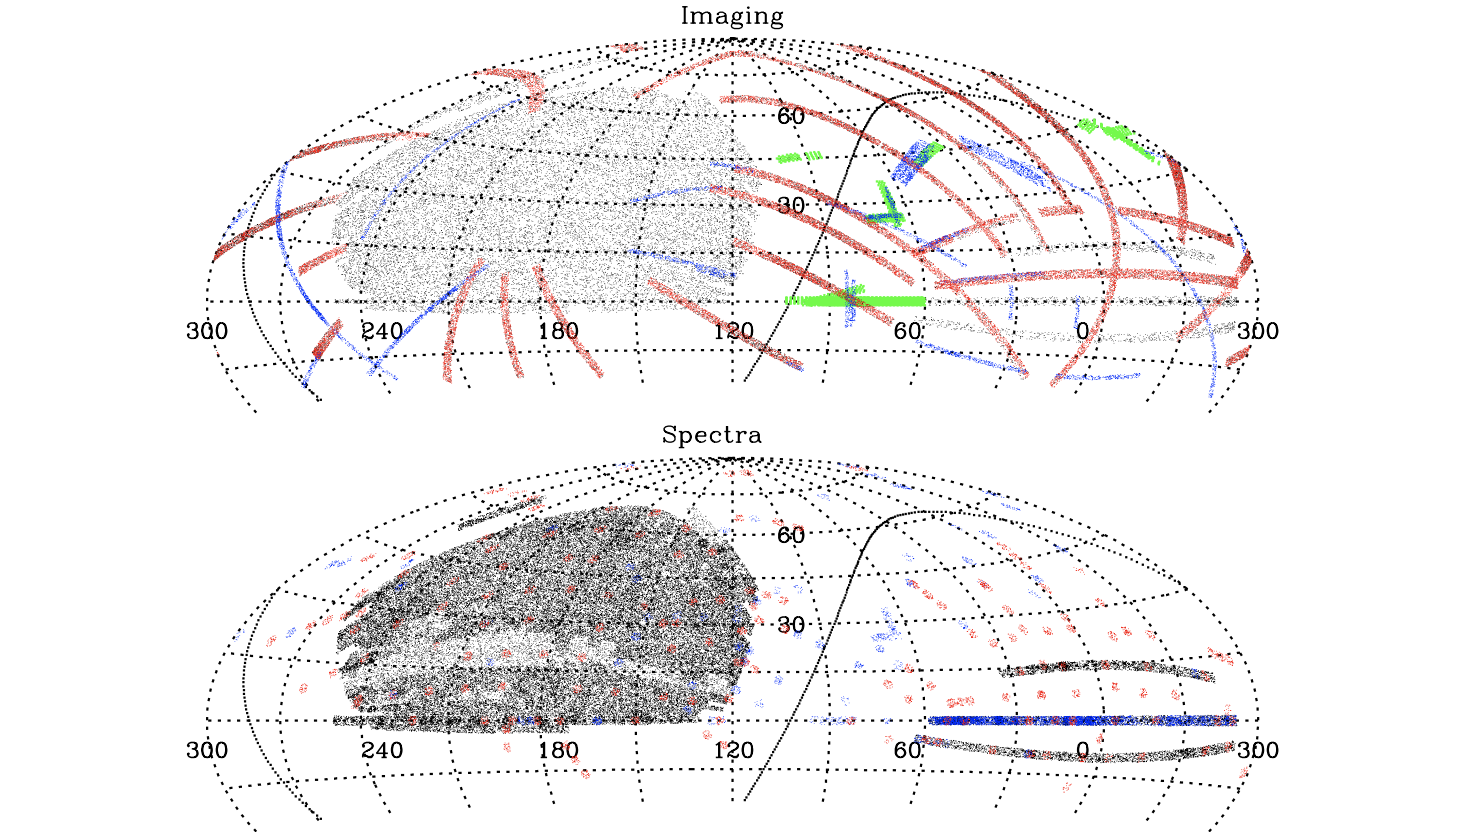
\includegraphics[width=0.8\textwidth]{SDSS_OFF}
  \caption{Regions of the sky surveyed by SDSS Data Release 7 \cite{2009ApJS..182..543A}}
  \label{3}
\end{figure}


\begin{comment}
 The first is a wide-field imager equipped with 24 tiles, each containing a 2048x2048 CCD. Imaging is performed along great circles at the sidereal rate, leading to exposure times of 54.1 seconds.

The astrometry is good to 45 milliarcseconds (mas) rms per coordinate at the bright end, while the photometric calibration is made in two modalities, respectively by tying to standard reference stars and by using the overlap between adjacent imaging runs in a process called ubercalibration.

Spectra are extracted and calibrated in terms of wavelength and flux. For galaxies near the main sample flux limit, the typical signal-to-noise ratio (S/N) is 10 per pixel. The broadband spectrophotometric calibration exhibits an accuracy of $4\%$ root mean square (rms) for point sources (Adelman-McCarthy et al. 2008), and the wavelength calibration is precise to $2 \, \text{km s}^{-1}$.

The SDSS data have been made public in a series of yearly data releases, This thesis works based its results from a galactic sample derived from "Data Release 7" by the Max Planck Institute for Astrophysics and Johns Hopkins University ( MPA-JHU )  teams, containing the derived properties of a total of 927'552 galaxy spectra.


\textbf{Physical Properties of interest :}
\begin{itemize}
		\item \textbf{Line Flux :}Flux from Gaussian fit to continuum subtracted data, corrected for foreground (galactic) reddening using techniques developed by O'Donnell \cite{1994ApJ...422..158O}
		\item \textbf{Error Line Flux :} Developed by analyzing the duplicate observations of galaxies, to compare the empirical spread in value determinations with the random errors.

\end{itemize}

\end{comment}


\subsection{C4 BCG Catalogue}
The identification of BCGs within our primary galaxy sample, previously described, relies on the findings of A. Von der Linden et al. \cite{2007MNRAS.379..867V, 2009yCat..73790867V}. These findings were derived from a subsequent analysis of the C4 Galaxy Cluster Catalog, initially developed by Miller et al. in 2005 \cite{2005AJ....130..968M}.

The C4 catalog comprises 748 galaxy clusters identified in the Second Data Release (DR2) of the Sloan Digital Sky Survey (SDSS). Utilizing a seven-dimensional position and color space, the C4 cluster-finding algorithm identifies overdensities. 

Covering approximately 2600 square degrees of the sky, the catalog spans redshifts from about 0.02 to 0.17. It includes various properties like sky location, mean redshift, galaxy membership, optical luminosity (Lr), velocity dispersion, and measures of substructure and large-scale environment.

This catalog represents one of the initial cluster catalogs constructed directly from SDSS spectroscopic data, addressing issues related to projection effects and employing mock galaxy catalogs derived from realistic N-body simulations to analyze the clustering algorithm's parameters and improve its completeness.

In this context, the work by Von Der Linden et al.  \cite{2007MNRAS.379..867V} is noteworthy, as it builds upon the C4 catalog but introduces improved algorithms for BCG identification and measuring cluster velocity dispersion,  ultimately yielding a sample of 625 BCGs.

Correcting for the SDSS photometric pipeline's tendency to underestimate luminosities in dense environments, the research refines the C4 galaxy cluster sample, addressing issues related to BCG luminosity underestimation. Given the challenges with SDSS photometry, especially for large galaxies in crowded areas, the study avoids using magnitude measurements assuming a specific profile shape.

The C4 catalog provides potential BCG candidates, but approximately $30\% $ of clusters miss the true BCG due to fiber collisions. To address this issue,  Von der Linden's team developed an algorithm to identify the BCG by estimating the virial radius, selecting the two brightest galaxies within the mean galaxy's projection, and assessing criteria such as concentration index, color compatibility, and redshift.

\subsection{The Radio Catalogue}
To investigate the radio emission characteristics of both BCGs and non-BCGs, this study conducted a crossmatch between the primary SDSS sample and a dataset comprising 2,712 radio-luminous galaxies from the work by \cite{2005MNRAS.362....9B}. This collection of radio-luminous objects resulted from a complex cross-matching process involving the main spectroscopic galaxy sample and two radio surveys: the National Radio Astronomy Observatories (NRAO) Very Large Array (VLA) Sky Survey (NVSS) \cite{1998AJ....115.1693C} and the Faint Images of the Radio Sky at Twenty centimeters (FIRST) survey. \cite{1995ApJ...450..559B}

The NVSS was the first radio survey with a sufficiently high angular resolution (45 arcsec) to allow automated cross-correlation with optical surveys. However, the FIRST catalogue offers superior angular resolution (approximately 5 arcsec), resulting in samples with much higher reliability. Nonetheless, the high angular resolution of FIRST presents its own challenges, as it is insensitive to extended radio structures and resolves out the extended emission of radio sources. Consequently, the total radio luminosity of sources larger than a few arcseconds is systematically underestimated by FIRST. To address these limitations, a hybrid approach utilizing both NVSS and FIRST surveys has been developed to identify radio sources associated with galaxies in the SDSS spectroscopic sample. This approach capitalizes on the sensitivity of NVSS to large-scale radio structures and the high angular resolution of FIRST to reliably pinpoint the host galaxy.

The obtained radio source sample demonstrated a completeness of $95\%$ and a reliability of $98.9\%$, upgrading the achievable performance of each individual survey. The sample was subsequently classified into two groups: radio-loud active galactic nuclei (AGN) and galaxies where radio emission is predominantly driven by star formation. Classification was based on a galaxy's position in the 4000-Å break strength versus radio luminosity per unit stellar mass plane, resulting in a dataset of 2,215 radio-loud AGN and 497 star-forming galaxies with radio luminosity exceeding 5 mJy at 1.4 GHz.

\begin{comment}
\vspace{3cm}
\begin{figure}[hbtp]
  \centering
  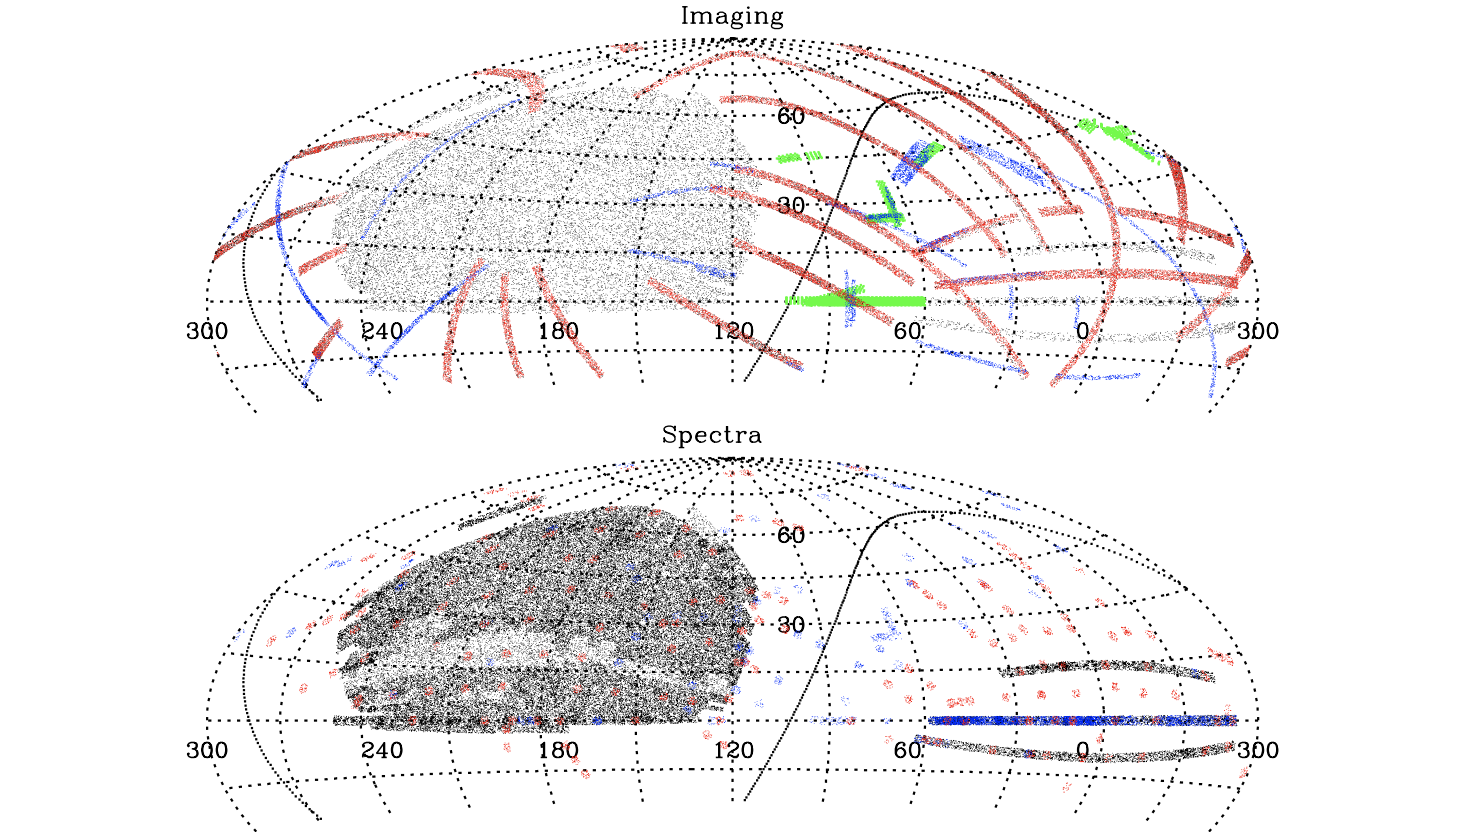
\includegraphics[width=0.8\textwidth]{SDSS_OFF}
  \caption{Regions of the sky surveyed by SDSS Data Release 7}
  \label{3}
\end{figure}
\end{comment}

\newpage
\section{Data Analysis}
As previously introduced, our primary galaxy sample for astrometry measurements is the MPA-JHU SDSS-derived catalogue.

The first operation required for the development of our study involved crossmatching the C4 BCG sample \cite{2009yCat..73790867V} to extract data files from the main sample, including both BCGs and non-BCGs.

This initial crossmatch was accomplished by selecting the nearest element within a radius of 2 arcsec in both RA and Dec corresponding to each of the BCGs in \cite{2009yCat..73790867V}. The result was a list of 484 corresponding selected elements.

At the end of this initial phase, the following data were collected for both samples:
\begin{itemize}
    \item \textbf{Astrometry data:} Celestial coordinates, Redshift, Error on redshift...
    \item \textbf{Spectroscopy measures:} Emission lines' fluxes and their relative errors
\end{itemize}

Even though further explanation is to follow, it is preferable to introduce the second crossmatch required for this work, this time with the 2712 galaxy samples of Celestial Objects found to be active in the radio field.

In this case, the research algorithm was designed to identify the nearest correspondence within a radius of 5 arcsec. The previously created files were appropriately updated by adding a specific flag, denoted as 1, to indicate whether, when found in the Radio Sample, it implies Radio Loud Emission.

\subsection{Optical analysis}
After previously introducing the defining properties of an AGN and discussing their effects on the host galaxy, it is crucial for the subsequent optical analysis of our two samples to examine which selected objects exhibit typical properties intrinsic to the presence of an AGN. One of the primary methods employed in Astrophysics is the analysis of BPT diagnostic diagrams \cite{1981PASP...93....5B}.

This type of analysis classifies different species of galaxies by scrutinizing specific ratios of emission lines produced by ionizing gas in the galaxy's Interstellar Medium (ISM), utilizing photoionization models. These specific ratios have been carefully chosen to prioritize similar wavelength fractions, minimizing dust attenuation. Specifically, this is developed based on the following ratios:
\begin{multicols}{2}
\begin{itemize}
    \item \textbf{$\frac{[OIII]\lambda 5007}{H\beta}$}
    \item \textbf{$\frac{[NII]\lambda 6583}{H\alpha}$}
    \item \textbf{$\frac{[SII]\lambda\lambda 6716,6731}{H\alpha}$}
    \item \textbf{$\frac{[OI]\lambda 6300}{H\alpha}$}
\end{itemize}
\end{multicols}

By examining these ratios, which provide evidence of different photoionization models, it is possible to draw demarcation lines and ultimately classify the final objects into different categories.

The underlying concept of this method is rooted in an intrinsic property of the ionization spectrum of massive stars near the Lyman limit of Helium, found at $\lambda = 228\AA$. Massive stars exhibit a bright cut, while the non-thermal radiation of AGNs extends to higher energies. 

As a result, AGN host galaxies typically show greater ratios that surpass the demarcation lines predicted by photoionization models.

There were several photoionization models at the inception of this technique; nowadays, the preferred ones are Kauffmann et al. \cite{2003MNRAS.346.1055K} and Kewley et al. \cite{2001ApJ...556..121K}.

While the ideal classification incorporates all three primary BPT diagnostics, this study relies on a classification derived solely from the BPT diagrams for [NII] and [SII].

\begin{itemize}
    \item \textbf{BPT-[NII] Demarcation Functions:}
    \begin{itemize}
        \item Kauffmann+03 Line: \[ \text{log}(\frac{\text{[OIII]}}{\text{H}\beta}) = 0.61 / (\text{log}(\frac{\text{[NII]}}{\text{H}\alpha}) - 0.05) + 1.3 \]
        \item Kewley+01 Line: \[ \text{log}(\frac{\text{[OIII]}}{\text{H}\beta}) = 0.61 / (\text{log}(\frac{\text{[NII]}}{\text{H}\alpha}) - 0.47) + 1.19 \]
    \end{itemize}

    \item \textbf{BPT-[SII] Demarcation Functions:}
    \begin{itemize}
        \item Main AGN Line: \[ \text{log}(\frac{\text{[OIII]}}{\text{H}\beta}) = 0.72 / (\text{log}(\frac{\text{[SII]}}{\text{H}\alpha}) - 0.32) + 1.30 \]
        \item LINER/Sy2 Line: \[ \text{log}(\frac{\text{[OIII]}}{\text{H}\beta}) = 1.89 \text{log}(\frac{\text{[SII]}}{\text{H}\alpha}) + 0.76 \]
    \end{itemize}
\end{itemize}

As follows it is presented a brief description of each population:

\begin{itemize}
    \item \textbf{BPT-[NII]:}

		\begin{itemize}
    		\item \textbf{Star-forming (SF):} Below both of the demarcation lines, where the ionization is primarily from massive stars.
    		\item \textbf{AGN (Active Galactic Nuclei):} Above both of the demarcation lines, delineating ionization by an active nucleus.
    		\item \textbf{Composite:} Galaxies exhibiting a mix of both star-forming and AGN characteristics. Generally recognized to be in the area between both of the demarcation lines.
		\end{itemize}

		\item \textbf{BPT-[SII]:}
	\begin{itemize}
    		\item \textbf{Seyferts:} Above of both of the demarcation lines, characterized by high ionization levels.
    		\item \textbf{LINERs (Low-Ionization Nuclear Emission Regions):} Above the Main AGN line, and below LINER/Sy2.  Typically characterized by weak AGN-like ionization.
    		\item \textbf{Star-forming HII2:} Galaxies exhibiting ionization characteristics similar to HII regions in star-forming galaxies.
		\end{itemize}

\end{itemize}


Returning to the methodology employed in this thesis, an initial screening process was conducted to exclude objects with flux values that rendered logarithmic ratios incalculable, specifically eliminating instances with numerators or denominators equal to zero. Subsequently, scatterplots were generated and demarcation lines were applied to discern distinct galaxy populations.
Results images can be seen in :

\autoref{4} \autoref{5} \autoref{6} \autoref{7}

Given the inclusion of error values for each flux measurement, a robust bootstrap algorithm was implemented through 5000 iterations. This algorithm introduced variations to each point on the diagnostic diagram in two dimensions based on its probability distribution, with the mean value reflecting the error-free point and a standard deviation equivalent to the error associated with the point in both directions.

This rigorous approach facilitated an accurate determination of counts and fractions for all populations, providing a statistically refined measure of uncertainty.
\vspace{2cm}
\begin{figure}[hbtp]
  \centering
  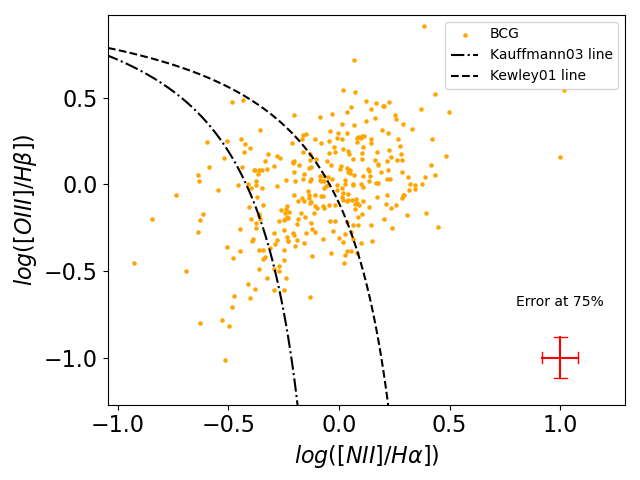
\includegraphics[width=0.65\textwidth]{BCG-NII-V22}
  \caption{BPT NII for the BCG sample }
  \label{4}
\end{figure}

\begin{figure}[hbtp]
  \centering
  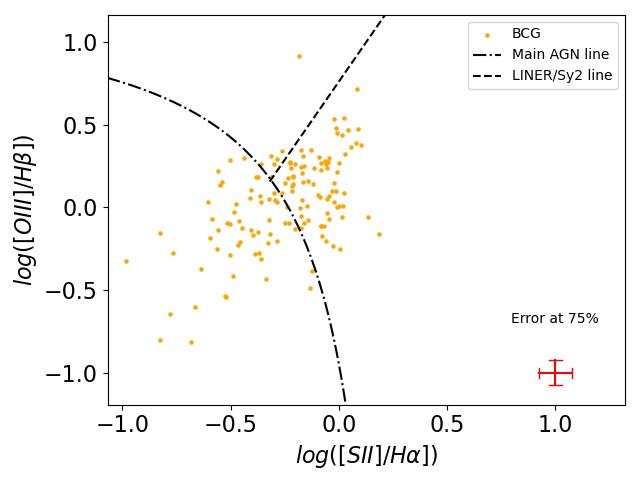
\includegraphics[width=0.65\textwidth]{BCG-SII1731-V22}
  \caption{BPT SII for the BCG sample }
  \label{5}
\end{figure}


\begin{figure}[hbtp]
  \centering
  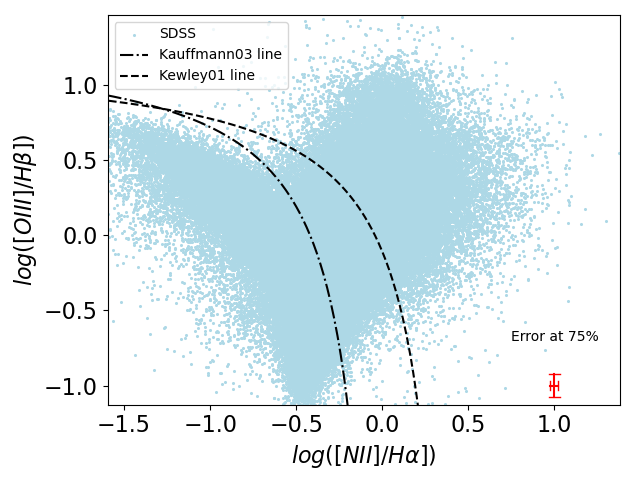
\includegraphics[width=0.7\textwidth]{SDSS-NII-V22}
  \caption{BPT NII for the SDSS noBCG sample }
  \label{6}
\end{figure}

\begin{figure}[hbtp]
  \centering
  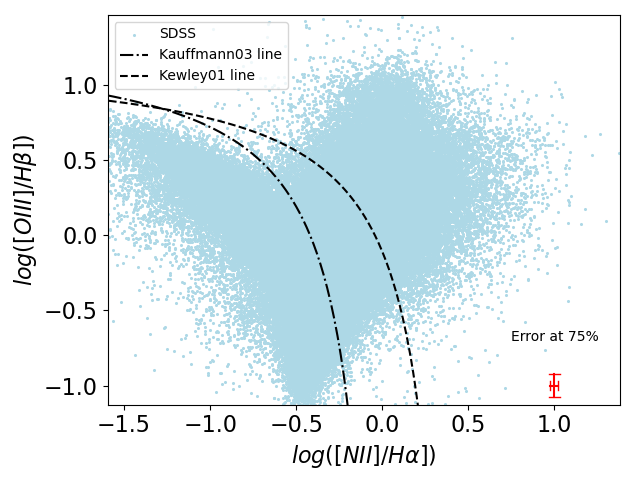
\includegraphics[width=0.7\textwidth]{SDSS-NII-V22}
  \caption{BPT SII for the SDSS noBCG sample }
  \label{7}
\end{figure}

\newpage
\subsection{Radio Analysis}

Following the preceding analyses, let's now detail how the fractions of Radio Loud AGNs were calculated for the two derived samples.

The primary goal of this analysis segment is to determine a fraction of the form :
 $$\frac{N_{\text{radio}}}{N_{\text{total}}}$$

A crucial step in calculating a representative fraction of Radio Loud objects was to appropriately define the spatial regions for the fraction calculations. To accomplish this, we identified the regions mapped by the radio survey employed. Subsequently, the selection has been delineated where all three catalogs exhibited an overlap. It is essential to emphasize that the primary objective is to obtain representative fractions for both of our samples.

The selected spatial regions considered for calculating the fractions of Radio Loud objects can be found in \autoref{8}

\vspace{2cm}
\begin{figure}[hbtp]
  \centering
  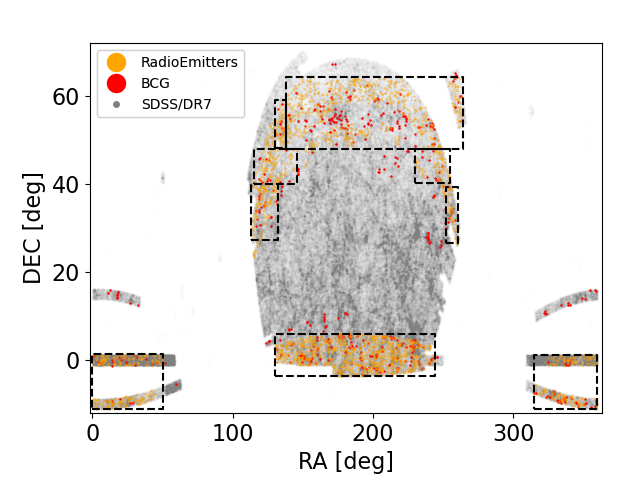
\includegraphics[width=0.9\textwidth]{Fourth}
  \caption{Defining Regions of Radio Loud AGN fractions }
  \label{8}
\end{figure}


 
